\documentclass[9pt]{article}
\usepackage{amsmath,amsfonts,amssymb,times}
\usepackage{graphicx,color,tikz,pgfplots}
\usepackage[paperwidth=16cm,paperheight=6.2cm,lmargin=0pt,rmargin=0pt,tmargin=0pt,bmargin=0pt]{geometry}
\usepackage{bm}
\usetikzlibrary{arrows,shadings,shapes.arrows,decorations.pathreplacing,calc}
\usepgfplotslibrary{fillbetween}


\pagestyle{empty}
\pgfplotsset{compat=newest}
\definecolor{applered}{RGB}{255,8,0}
\definecolor{azure}{RGB}{0,127,255}
\definecolor{violet}{RGB}{159,0,255}

\pgfdeclareverticalshading{rainbow}{100bp}
{color(0bp)=(applered); color(25bp)=(red); color(40bp)=(yellow);
  color(47bp)=(green); color(51bp)=(cyan); color(60bp)=(blue);
  color(65bp)=(violet); color(100bp)=(violet)} 
                          
\newlength{\h}
\newlength{\rad}
\setlength{\h}{1.5cm}
\setlength{\rad}{1.0pt}

\begin{document}
\centering
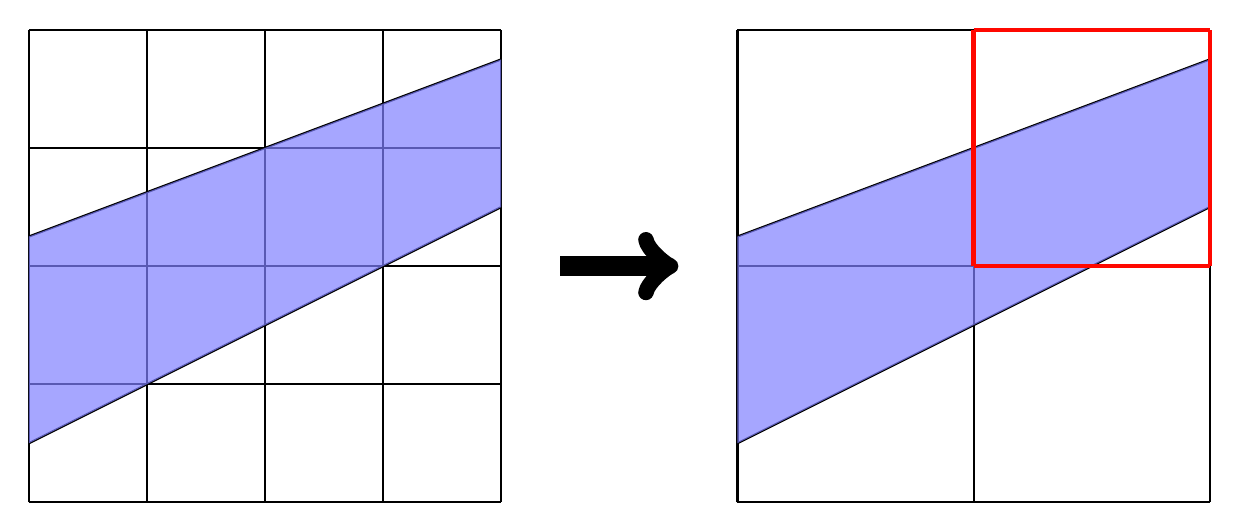
\begin{tikzpicture}[
    gridstyle/.style={thick,black},
    surfaceFill/.style={},
  ]

  % Fine grids
  \draw[step=\h,gridstyle] (0,0) grid (4\h,4\h);
  \draw[thick, black, name path=lo] (0, 0.50\h) -- (4\h, 2.5\h);
  \draw[thick, black, name path=hi] (0, 2.25\h) -- (4\h, 3.75\h);
  \tikzfillbetween[of=lo and hi,on layer=,every segment/.style={surfaceFill}] {opacity=0.7, blue!50!white};

  \draw[ultra thick, line width=7pt, ->] (4.5\h, 2\h) -- ++ (1\h, 0);
  % Coarsened grids
  \begin{scope}[xshift=6\h]
    \draw[step=2\h,gridstyle, draw=black, thick] (0\h,0\h) grid (4\h,4\h);
    \draw[thick, black, name path=lo] (0\h, 0.50\h) -- (4\h, 2.5\h);
    \draw[thick, black, name path=hi] (0, 2.25\h) -- (4\h, 3.75\h);
    \tikzfillbetween[of=lo and hi,on layer=,every segment/.style={surfaceFill}] {opacity=0.7, blue!50!white};
    \draw[step=2\h,gridstyle, draw=applered, ultra thick] (2\h,2\h) grid (4\h,4\h);
  \end{scope}

  %% %EB
  %% \path[name path=baseline] (1.5\h,\h) -- (3\h,\h);
  %% \draw[surfaceStyle,name path=surface] (1.5\h,\h) -- (2\h,1.5\h) -- (3\h,1.75\h);
  %% \tikzfillbetween[of=surface and baseline,on layer=,every segment/.style={surfaceFill}] {black!50!white};

  %% %% Grids and nodes
  %% \draw[step=\h,gridstyle] (0,\h) grid (3\h,3\h);
  %% \draw[nodeCenterStyle] (1.5\h, 1.5\h) circle(\rad) node[phiStyle, below] {$(i,j)$};

  %% % Flux right face
  %% \draw[nodeFaceStyle]   (2.0\h, 1.75\h) circle (\rad) node[phiStyle] {};
  %% \draw[normalStyle]     (2.0\h, 1.75\h) --++ (0.5\h, 0.0\h) node[phiStyle,right] {$F_2$};

  %% % Flux left face
  %% \draw[nodeFaceStyle]   (1.0\h, 1.5\h) circle (\rad) node[phiStyle] {};
  %% \draw[normalStyle]     (1.0\h, 1.5\h) --++ (-0.5\h, 0.0\h) node[phiStyle,left] {$F_1$};

  %% % Flux top face
  %% \draw[nodeFaceStyle]   (1.5\h, 2.0\h) circle (\rad) node[phiStyle] {};
  %% \draw[normalStyle]     (1.5\h, 2.0\h) --++ (0.0\h, 0.5\h) node[phiStyle,above] {$F_3$};

  %% % Boundary flux
  %% \draw[nodeFaceStyle]   (1.25\h, 1.0\h) circle (\rad) node[phiStyle] {};
  %% \draw[normalStyle]     (1.25\h,  1.0\h) --++ (0.0\h, -0.5\h) node[phiStyle,below] {$F_{\text{D}}$};

  %% % EB flux
  %% \draw[nodeFaceStyle]   (1.75\h, 1.25\h) circle (\rad) node[phiStyle] {};
  %% \draw[normalStyle]     (1.75\h, 1.25\h) --++ (+0.5\h, -0.5\h) node[phiStyle,below,right] {$F_{\text{EB}}$};

%%   \foreach \x in {\h/2,3\h/2,5\h/2} {
%%     \foreach \y in {\h/2,3\h/2,5\h/2} {
%% %      \draw[nodeCenterStyle] (\x,\y) circle (\rad);
%%     }
%%   }
  %% \foreach \x in {\h/2,3\h/2,5\h/2} {
  %%   \foreach \y in {0,\h,2\h,3\h} {
  %%     \draw[nodeCenterStyle] (\x,\y) circle (\rad);
  %%   }
  %% }
  %% \foreach \x in {0,\h,2\h,3\h} {
  %%   \foreach \y in {\h/2,3\h/2,5\h/2} {
  %%     \draw[nodeCenterStyle] (\x,\y) circle (\rad);
  %%   }
  %% }


  %% Dielectric surface


  %%\draw[braceStyle] (1.35\h,\h) -- (2\h,1.4\h) node [EBStyle,midway,above] {$\alpha_{\bm{i}}^{\text{EB}}$};
  %%\draw[normalStyle] (1.5\h,1.1\h) -- (1.4\h,1.275\h) node [above] {$\hat{\bm{n}}_{\bm{i}}^{\text{EB}}$};

  %% Surface fractions
  %% \draw[braceStyle] (2\h,2\h) -- (2\h,1.4\h) node [midway,right = 1em,alphaStyle,anchor=west] {$\alpha_{\bm{i}+\frac{1}{2}\bm{e}_0},\,\overline{\bm{x}}_{\bm{i}+\frac{1}{2}\bm{e}_0}$};
%%  \draw[nodeFaceStyle] (1.35\h,1.6\h) circle (\rad) node[phiStyle] {};%$\overline{\bm{x}}_{\bm{i}},\,\kappa_{\bm{i}}$};
  %% \node[phiStyle] at (1.5\h,1.5\h) {$\bm{x}_{\bm{i}}$};
  %% \draw[braceStyle] (\h,3\h) --++ (\h,0) node[midway,above,hTopStyle,anchor=south] {$\Delta x$};
  %% \draw[braceStyle] (0,\h) --++ (0,\h) node[midway,left,hLeftStyle,anchor=east] {$\Delta x$};


  
\end{tikzpicture}
\end{document}
